%\chapter{det-comp}


%%%%%%%%%%%%%%%%%%%%%%%%%%%%%%%%%%%%%%%%%%%%%%
%\section{Anode Plane Assemblies}

%%%%%%%%%%%%%%%%%%%%%%%%%%%%%%%%%%%%%%%%%%%%%%
\section{Cathode Plane Assemblies (CPA)}
\label{sec:cpa}

%\subsection{Scope, requirements and design considerations}
\subsection{Scope and requirements}

\fixme{Need to clarify language: One CPA plane (7m x 6m) made up of six CPAs (or CPA columns), each CPA made up of 3 vertically stacked CPA modules. Each module made up of resistive panel in frame. Anne to do.}

The cathode plane is located in the middle of the TPC, dividing the detector into two equal-distance drift volumes. The cathode plane's 7\,m $\times$ 6\,m area is made up of six columnar \textit{cathode plane assemblies (CPAs)}, each of which is constructed of three vertically stacked \textit{CPA modules}. The cathode plane therefore consists of 18 CPA modules. 

The cathode plane is connected to the high voltage feedthrough through a receptacle, called the \textit{HV cup}, at the east end, \fixme{Saleve side?} and biased at $-$180\,kV.   It provides the bias voltage and current to all the field cage modules (top, bottom and end walls) (Section~\ref{detcompsec-fc}) through electrical interconnects.  It also mechanically supports six pairs of top/bottom field cage modules. The cathode plane is suspended by insulating bars from the CPA installation rail.

%  It is connected to the high voltage feedthrough through a receptacle, called the \textit{HV cup}, at the east end, \fixme{Saleve side?} and biased at $-$180\,kV.  The cathode plane is constructed from six columnar cathode plane assemblies (CPAs) to form the 7\,m $\times$ 6\,m area.  It provides the bias voltage and current to all the field cage modules (top, bottom and end walls) through electrical interconnects.  It also mechanically supports six pairs of top/bottom field cage modules. The cathode plane is suspended by insulating bars from the CPA installation rail.

\fixme{Gina underlined `bias' in `bias voltage' above and in first bullet point; not sure why (Anne)}

%%%%%%%%%%%%%%%%%%%%%%%%%
%\subsubsection{Requirements}
The CPA plane is required to:
\begin{itemize}
\item provide equipotential surfaces at $-$180kV nominal bias voltage,
\item maintain a flatness better than 1~cm when submerged in the liquid argon,
\item be constructed of materials with comparable CTEs to that of stainless steel, 
\fixme{CTE coeff of therm expansion -- add to acronym list}
\item limit the electric field exposed to LAr to under 30~kV/cm 
\item prevent damage to the TPC, including its readout electronics, in case of a HV discharge anywhere on the cathode,
\item provide constant bias voltage and current to all attached field cage (FC) resistor divider chains,
\item support the full weight of the four connected top/bottom field cage modules plus a person on the bottom CPA \fixme{CPA or FC?} during installation,
\item accommodate cryostat roof movement between warm and LAr-filled states,
\item be constructed in a modular form that can be easily installed in the cryostat,
\item accommodate Photon Detection System (PDS) calibration features, and
\item avoid any trapped volume of LAr.
\end{itemize}

%%%%%%%%%%%%%%%%%%%%%%%%%
\subsection{Design considerations}

%In a single phase DUNE far detector module, the cathode planes are planned to be 12\,m tall by nearly 60\,m long.  When biased to the nominal voltage of $-$180\,kV, each cathode plane stores more than 100\,J of energy. It is of great concern on the integrity of the detector elements, including the sensitive front end electronics, if this energy is suddenly and completely released in a high voltage discharge event.  Study has shown (DUNE docdb 1320) \fixme{cite properly} that if the entire cathode plane is made of interconnected metallic electrodes, there is significant risk of damage to the front end ASICs simply due to the charge injection through the capacitive coupling between the cathode and the anode wires when the cathode voltage is forced to ground by a high voltage discharge.  

In a single phase DUNE far detector module, the cathode planes are planned to be 12\,m tall by nearly 60\,m long.  When biased to the nominal voltage of $-$180\,kV, each cathode plane stores more than 100\,J of energy. If this energy were to be released  suddenly and completely in a high-voltage discharge event, it could greatly affect the integrity of the detector elements, including the sensitive front-end electronics.  
Study has shown (DUNE docdb 1320) \fixme{cite properly} a cathode plane made of interconnected metallic electrodes would present significant risk to the front-end ASICs due to the charge injection through the capacitive coupling between the cathode and the anode wires in such an event.  

%Since  a large fraction of the stored energy on the cathode plane is determined by the operating voltage and the drift distance, reducing the drift distance and therefore the cathode voltage is an option.  However, doing so while maintaining a constant detector fiducial volume would require additional detector elements and increase cost and complexity of the system.  And this will not reduce the amount of charge injection since the voltage-capacitance product remains nearly constant between the anode and cathode planes.

%Subdividing the cathode into electrically isolated partitions also reduces the total energy from a single cathode partition. However the capacitive coupling between wires and cathode will not change substantially until the partition size is comparable to the drift distance. Multiple HV feedthroughs and ports per cathode also increases the system complexity. Complete HV isolation of the cathode segments is a difficult task to achieve, if the cathode plane is also required to introduce little distortion in the drift field during normal operation of the detector. 

%The solution adopted in the single phase TPC design is to make the entire cathode plane out of highly resistive material such that it has a very long discharge time constant compared to an all metal construction.  In an event of high voltage breakdown at any given location on the cathode, the sudden change in voltage only occurs in a relatively localized area.  The rest of the cathode surface maintains its original bias voltage, and gradually discharges to ground through the large resistivity of the cathode material.  This greatly reduces the instantaneous charge injection to the front end electronics.

Among the possible solutions, the single-phase TPC design has adopted one in which the entire cathode plane is made out of highly resistive material such that it has a very long discharge time constant compared to an all metal construction.  In the event of HV breakdown at a given location on the cathode plane, the sudden change in voltage is restricted to the CPA module in question, \fixme{true?} a relatively localized area.  The rest of the cathode plane maintains its original bias voltage, and gradually discharges to ground through the large resistivity of the cathode material.  This greatly reduces the instantaneous charge injection to the front-end electronics.


%%%%%%%%%%%%%%%%%%%%%%%%%
\subsection{CPA plane design}

%%%%%%%%%%%%%%%%%%%%%%%%%
%\subsubsection{Overview}

%The cathode plane design has evolved through several iterations over the years.  The design chosen for the ProtoDUNE-SP TPC is an array of moderately sized modules constructed from strong FR4 (the fire-retardant version of G10) frames holding thin FR4 sheets laminated with a commercial resistive Kapton film on both sides.   Compared with the size of an APA, the CPA modules are 1/2 in width (1.16\,m) and 1/3 in height (2\,m).   Each module has four FR4 bars holding a 3mm thick FR4 sheet with resistive coating.  The thickness of the FR4 bars is 6cm.  The surfaces of the bars facing the APAs are covered by another set of resistive FR4 strip with a different bias voltage such that these FR4 bars do not cause any distortion in the drift field beyond the resistive surfaces.

The cathode plane design chosen for the ProtoDUNE-SP TPC is an array of 18 moderately sized modules constructed from strong FR4 (the fire-retardant version of G10) frames holding thin FR4 sheets laminated with a commercial resistive Kapton film on both sides.   Compared with the size of an APA, the CPA modules are 1/2 in wide (1.16\,m) and 1/3 in high (2\,m).  
\fixme{this makes no sense to me.  There is no such thing as an APA module, therefore we should compare APA to CPA, not to CPA module. What's with the 1/2 in and 1.16 m? I vote to delete prev sentence.}

Each module has four FR4 bars holding a 3-mm-thick FR4 sheet with resistive coating.  The thickness of the FR4 bars is 6~cm. 
\fixme{clarify bar versus sheet}
 The surfaces of the bars facing the APAs are covered by another set of resistive FR4 strips with a different bias voltage such that 
 %these FR4 
 the bars cause no distortion in the drift field beyond the resistive surfaces.


A CPA is constructed from the three CPA modules, forming a single column. \fixme{compare sizes here} Each CPA is suspended under the cathode support rail by a single insulating FR4 bar.  On the top and bottom edges of a CPA, there are two hinges supporting the partial weight of the top and bottom field cage modules.   Adjacent CPAs are aligned through pin-and-slot connections to maintain co-planarity while allowing minor relative vertical shift due to cryostat roof movement.

The electrical connectivity of the resistive panels vertically along each CPA is maintained by several tabs through the edge frames.  Across the columns, there is no direct electrical connection between the panels.  Instead, they are interconnected by the ``high-voltage bus''. 

The high-voltage bus is a loop of a HV cable placed along the outer edges of the entire cathode plane, hidden between the field-shaping strip overhang and the main cathode resistive sheet.  This cable must be capable of withstanding the full cathode bias voltage to prevent direct arcing to (and as a result, recharging) a cathode panel having a discharge to ground. 
\fixme{clarify previous sentence} The HV bus makes redundant connections to the resistive panels across CPAs. \fixme{but only at the top and bottom?}  It also provides a low-resistance path for the field cage resistive divider chains around the cathode edges.

The outer edges of the cathode plane facing the cryostat wall are populated with the same metal profiles, with insulating polyethylene caps, as used in the field cage.  This eliminates the need for a special design of the most crucial regions of the cathode plane: the edges of the CPA now look just like a continuation of the field cage.  Since these profiles are the only objects facing grounded surfaces, they are the most likely candidates to have HV discharges to ground.   To limit peak current flow, these edge profiles are resistively connected to the main cathode panels through their laminated resistive surfaces.  

\begin{cdrfigure}[Resistive surface CPA concept]{cpa-concept}{The resistive surface CPA concept showing  
 a 3D model of a corner of the cathode with major components.} 
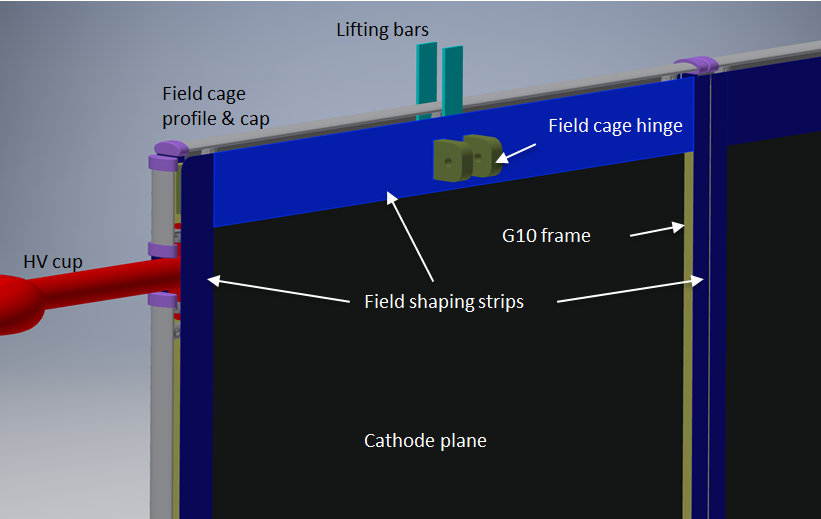
\includegraphics[width=\linewidth]{tpc_cpa_concept_leftonly}
\end{cdrfigure}

\fixme{figure \ref{fig:cpa-concept} is not referenced}


%%%%%%%%%%%%%
%\subsubsection{Resistive material}

The main criteria for the selection of the resistive material to be used for the CPA modules are: 
\begin{itemize}	
\item surface resistivity range,
\item compatibility with cryogenic temperatures,
\item robustness to HV discharges, 
\item material ageing,
\item radio-purity,
\item availability on large area, \fixme{in large enough panels?} and 
\item flatness, per the cathode flatness requirement. 
\end{itemize}

\fixme{What material was chosen?} 

%%%%%%%%%%%%
%\subsubsection{Support frame} % material properties}


Figures~\ref{fig:cpa-geometry} and~\ref{fig:cpa-view2} show the basic geometry of the cathode plane. Figure~\ref{fig:cpa-view2}a shows the block at the top of a CPA that is secured to the top cross bar and extends to the top supporting I-beam.  This strap \fixme{strap? not block or cross bar or I-beam?} must support the weight of four half FCs (4 $\times$ 220~lbs) and the weight of the CPA itself (160~lbs) for a total weight of 1,041~lbs. \fixme{What do the lower two images show?} Figure~\ref{fig:cpa-hinge1} shows how the FC is attached to the assembled cathode plane. 

\begin{cdrfigure}[CPA geometry]{cpa-geometry}{Basic geometry of the CPA array, close ups and a CPA column (on its side)} 
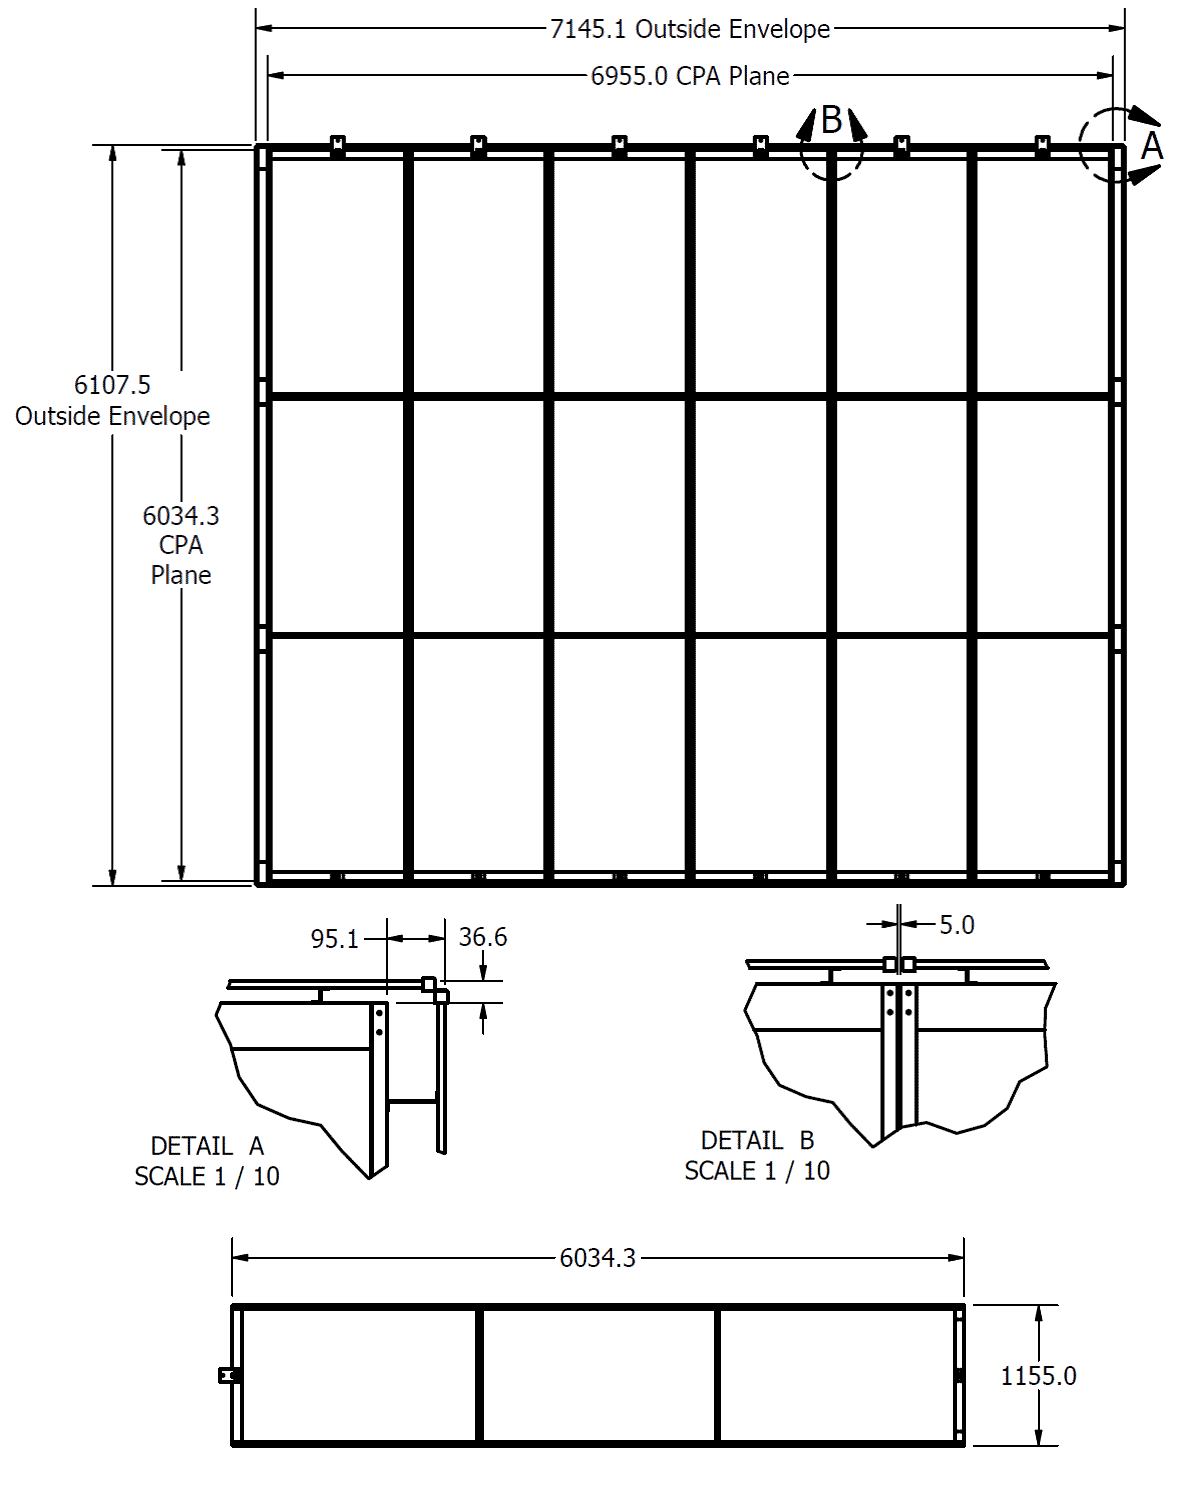
\includegraphics[width=\linewidth]{tpc_cpa_front_views1.png}
\end{cdrfigure}

\begin{cdrfigure}[CPA views2]{cpa-view2}{Views of various part of a CPA} 
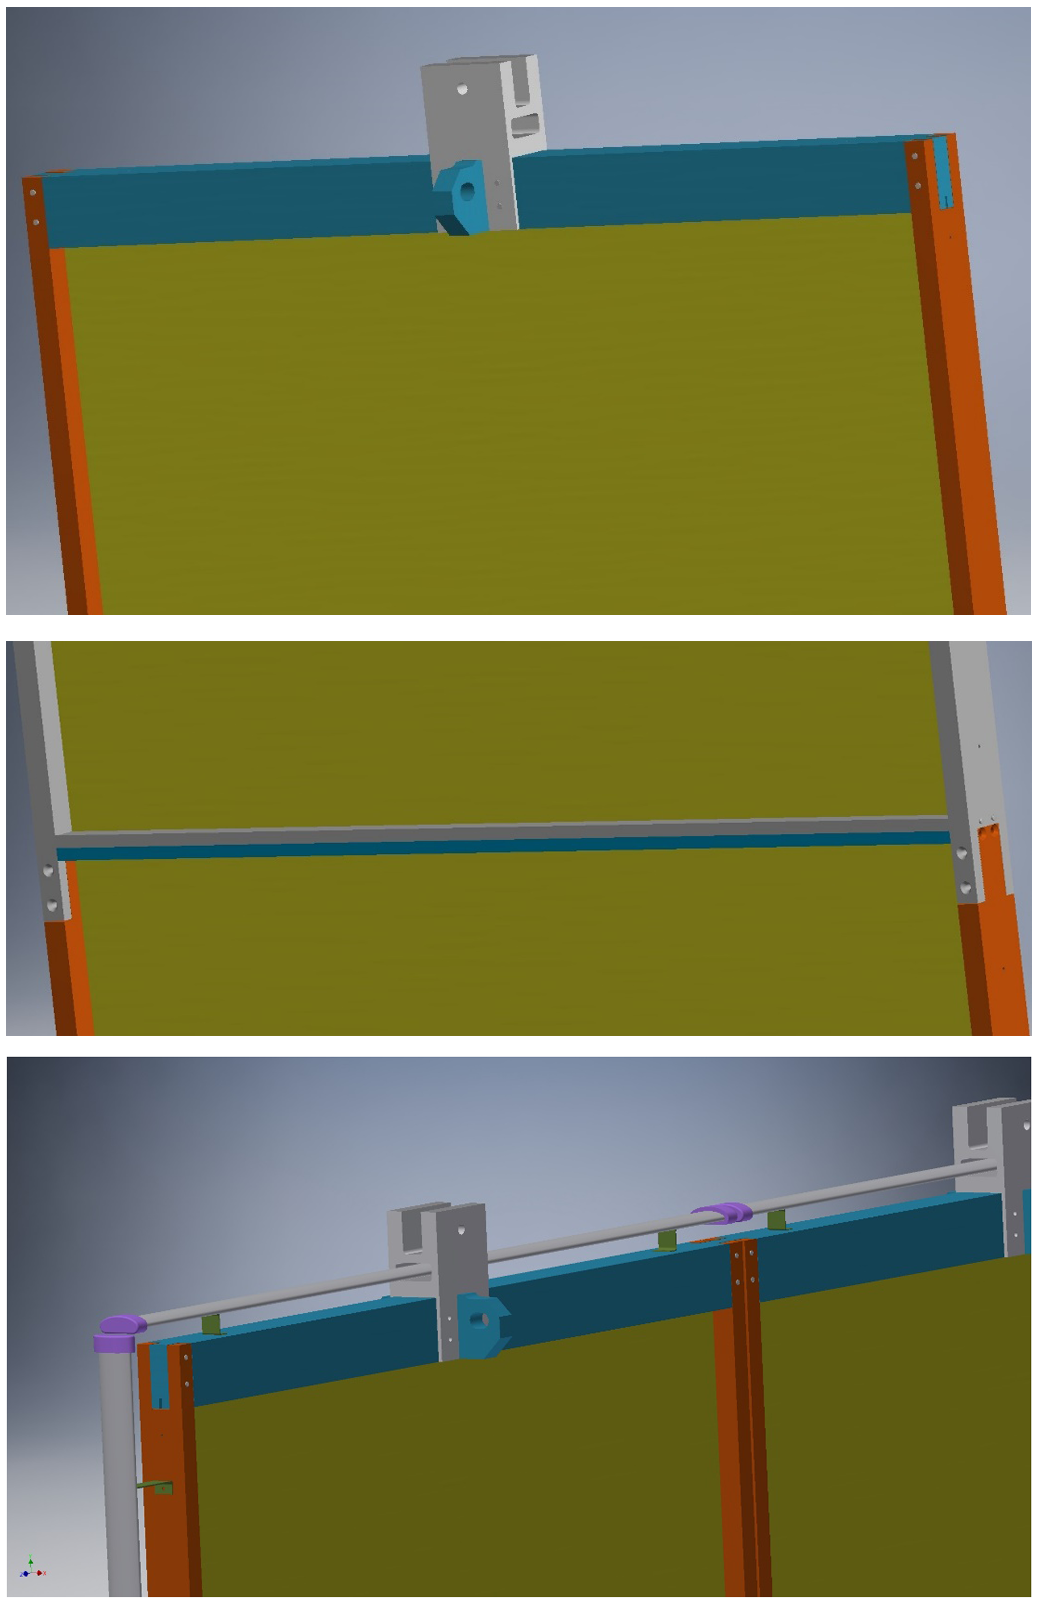
\includegraphics[width=0.8\linewidth]{tpc_cpa_views2.png}
\end{cdrfigure}

\begin{cdrfigure}[CPA and FC module hinged connection]{cpa-hinge1}{The top field cage modules are hung vertically with the CPAs when moved into the cryostat, then rotated to horizontal to attach to the APA.} 
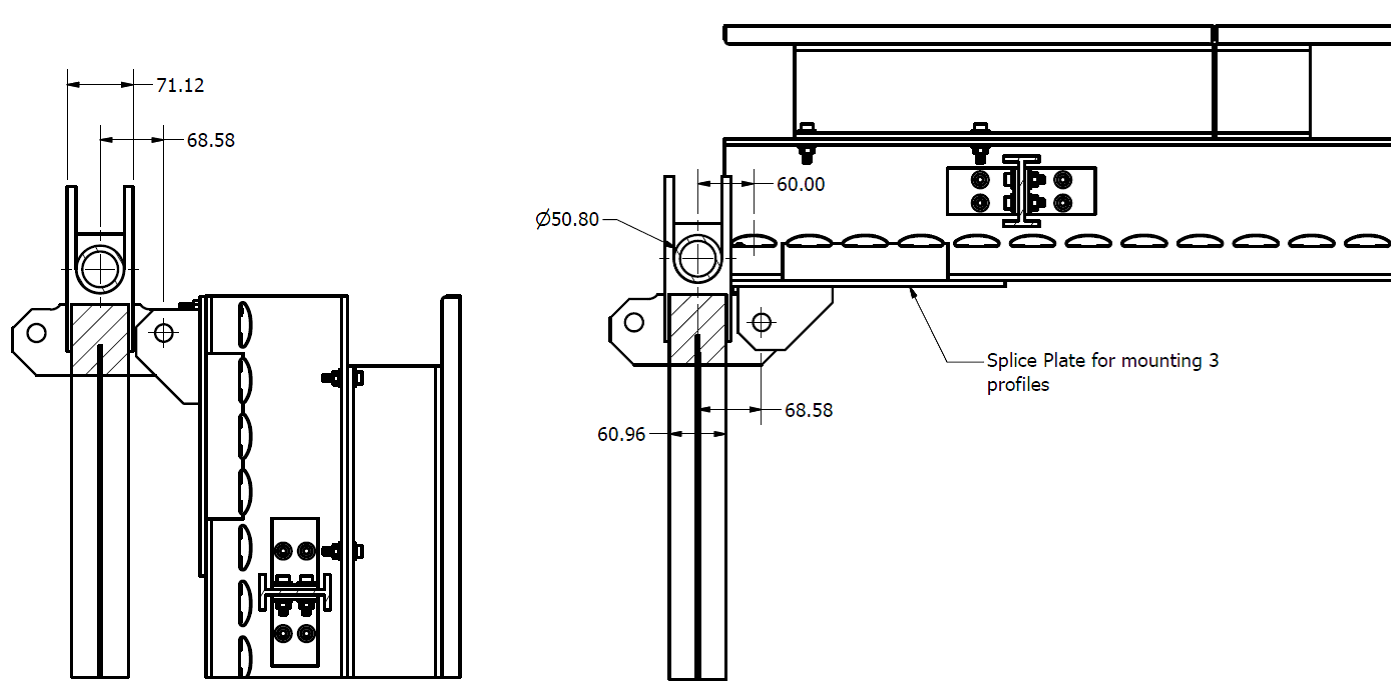
\includegraphics[width=\linewidth]{tpc_cpa_fc_hinge.png}
\end{cdrfigure}


{\it Deformation and stress due to pressure from circulating LAr}

Calculations %done at Fermilab 
indicate that a uniform 2~Pa pressure during cool down will be
\fixme{should be?}
  applied to the resistive panels  and that this will result in 0.090~inch deflections of the panel at its center.  The CPA/FC/APA assembly will displace 8.8~mm laterally as a result of the net force from this pressure.  \fixme{Is there such a thing as a CPA/FC/APA assembly?}

{\it Thermal considerations}

When the CPA modules are cooled, their width will shrink by 0.9~mm.  The supporting stainless steel beam will shrink by 1.6~mm over the width of the CPA.  If the CPA supports are rigidly attached to the supporting stainless steel beam, then an interference of 0.7~mm (the difference) will occur.  To prevent this interference and ensure contact between CPAs after cooldown, an initial gap of 0.7~mm between CPAs is required.  

The steel beam between the CPA and APA will shrink by 5.2~mm relative to the field cage length when cooled to LAr temperature.  The joint between the FC and the CPA must be able to accommodate this shrinkage.



%%%%%%%%%%%%
\subsection{Mechanical and electrical interconnections between modules}

Three modules are stacked vertically to form the 6-m height of a CPA. %the ProtoDUNE-SP  cathode.  
The frames of these modules are bolted together using tongue-and-groove connections at the ends. The resistive cathode sheets and the field-shaping strips are connected using a few metallic buttons to ensure redundant electrical contact between the CPAs. %vertical modules. 
\fixme{are the ``buttons'' called something else in the figures? }

%There are six 6\,m tall CPA modules in  ProtoDUNE-SP.  
Each CPA is suspended from the cathode rail using a central lifting bar.  Due to the roof movement between the warm and cold phases of the cryostat as it is cooled, each CPA is expected to move $\sim$2~mm relative to its neighbors.  Several pin-and-slot connections are implemented at the long edges of the CPA columns to ensure the co-planarity of the modules and yet allow small vertical displacement.  A low-resistance
``high voltage bus''  interconnects the resistive cathode surfaces across the columns to maintain a uniform voltage across the cathode surface.

The HV bus provides the high voltage to the FC
circuit and cathodes with a voltage drop much less than 0.1\% of the
cathode voltage. The location of the bus with respect to the CPA frame is shown in Figure~\ref{fig:HVbusmodel}. Field-shaping electrodes on the faces of the CPA
frames \fixme{on the face of the frames? does this mean on the side of the frame parallel to the resistive panel?} are part of the FC circuit, described in Section~\ref{detcompsec-fc}. 
FC electrodes on the outer edges of the
CPA frames \fixme{the part facing up in the figure?} are held at the cathode potential to provide field
uniformity and to protect the HV bus from discharge.  The feedthrough
connects to a HV cup on one side of a CPA at one end of
the cathode plane.  Interconnection of the bus between CPAs is made
through HV cables passed through the CPA frames. 

\begin{cdrfigure}[Model of the HV bus]{HVbusmodel}{A perspective view of CPA frame showing the location of the HV bus cable and attachments to the HV cup and resistive cathode, with CPA frame electrodes omitted to make HV bus visible.}
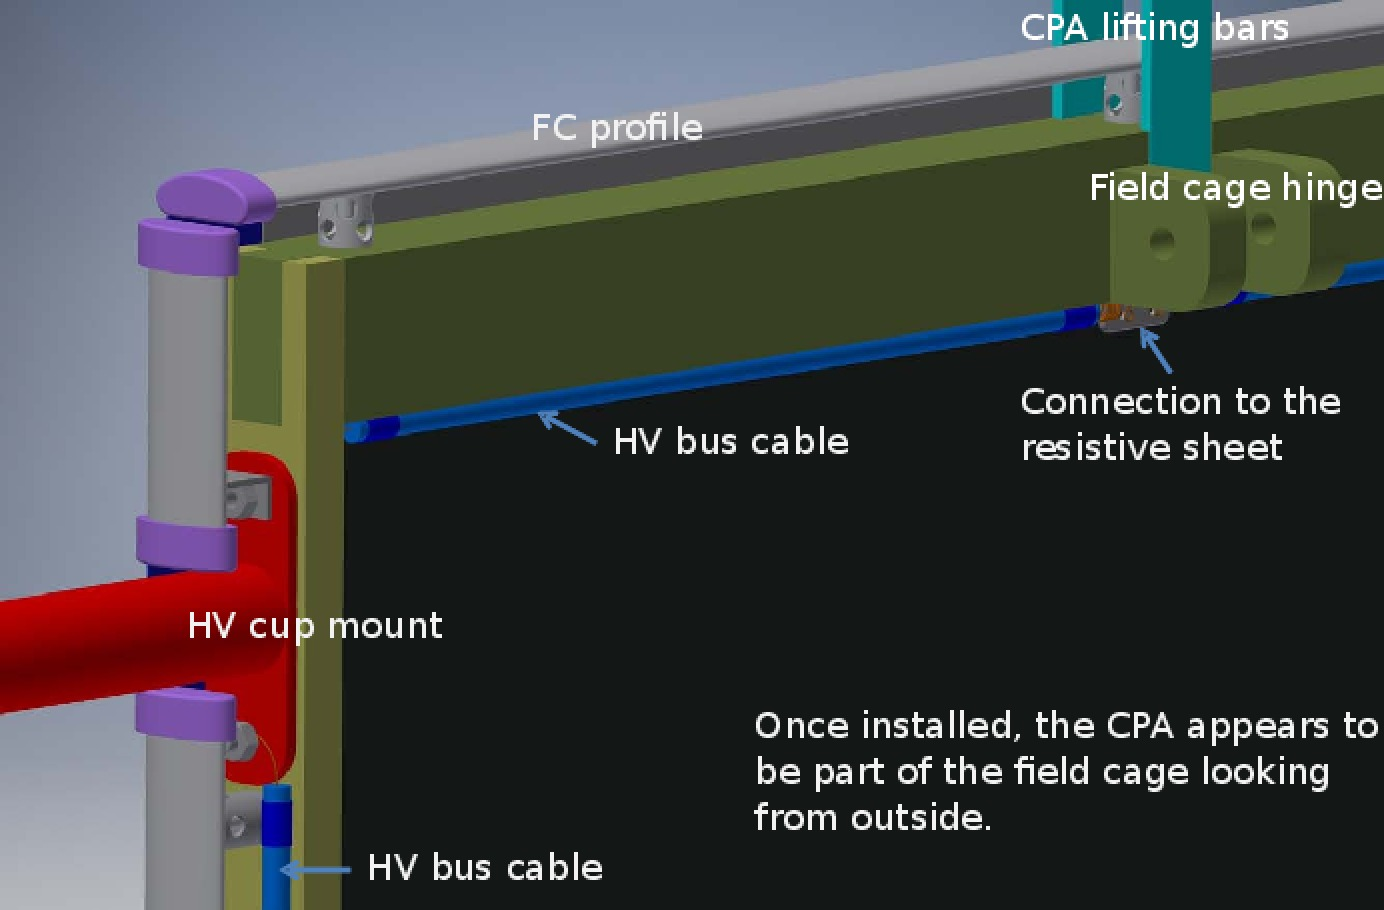
\includegraphics[height=0.35\textheight]{DUNE_SP_CPA_Design_Update-slide17-mod}
\end{cdrfigure}


